\documentclass{article}
\usepackage[T1]{fontenc}
\usepackage{lmodern}
\usepackage{graphicx}
\usepackage{amsmath,amssymb}
\usepackage[a4paper,margin=2cm]{geometry}
\usepackage[absolute,overlay]{textpos}
\setlength{\TPHorizModule}{1mm}
\setlength{\TPVertModule}{1mm}
\usepackage[indonesian]{babel}
\usepackage{hyperref}
\setlength{\emergencystretch}{2em}
% unit: Halaman 7

\begin{document}

% === Halaman 7 (llm) ===

\begin{itemize}
  \item Misalkan $e$ dan $d$ dipilih sedemikian sehingga
  \[ e \cdot d \equiv 1 \pmod{\phi(n)} \]
  atau
  \[ e \cdot d = k\phi(n) + 1 \]
  Maka
  \[ m^{k\phi(n)+1} \equiv m \pmod{n} \]
  \vspace{5mm}
  \[ m^{e \cdot d} \equiv m \pmod{n} \longrightarrow (m^e)^d \equiv m \pmod{n} \]
  \vspace{5mm}
  \item Enkripsi: $c = E_e(m) = m^e \pmod{n}$
  \item Dekripsi: $m = D_d(c) = c^d \pmod{n}$
\end{itemize}

\vspace{32.97mm}

% deskripsi: Persamaan enkripsi RSA yang dilingkari kotak merah
% bbox normalisasi: [0.2470, 0.6340, 0.5300, 0.7450]
\begin{textblock*}{59.43mm}(51.87mm,188.30mm)
\noindent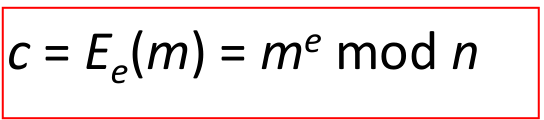
\includegraphics[width=59.43mm,height=32.97mm]{../../images/llm/page_007_img_01.png}%
\end{textblock*}

% deskripsi: Persamaan dekripsi RSA yang dilingkari kotak merah
% bbox normalisasi: [0.2470, 0.7610, 0.5320, 0.8720]
\begin{textblock*}{59.85mm}(51.87mm,226.02mm)
\noindent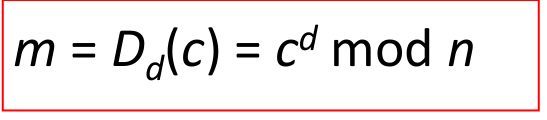
\includegraphics[width=59.85mm,height=32.97mm]{../../images/llm/page_007_img_02.png}%
\end{textblock*}

\end{document}
